%---Packages---%
\documentclass[a4paper,11pt]{article}
\usepackage[left=2.5cm,top=2cm,right=2cm,nohead]{geometry}
\usepackage[french]{babel}
\usepackage[T1]{fontenc}
\usepackage[utf8]{inputenc} 
\usepackage{graphicx}
\usepackage{float}
\usepackage{amsmath}
\usepackage{amsfonts}
\usepackage{amssymb}
\usepackage{listings}
\usepackage{mdwlist}
\usepackage[usenames,dvipsnames]{color}
\usepackage[stable]{footmisc}%To include footnotes in 'section' parts
\usepackage{hyperref}
\usepackage{setspace}
\usepackage{eurosym}
\usepackage[section]{algorithm} % [section] is use to define the numbering mode
\usepackage{algorithmic} 

%---Insertion de code---%
\definecolor{lightgray}{gray}{0.95}


\lstset
{           
backgroundcolor=\color{lightgray},
keywordstyle=\color{Red}\bfseries,
ndkeywordstyle=\color{darkgray}\bfseries,
commentstyle=\color{Green},
stringstyle=\color{Orange},
basicstyle=\footnotesize,       % the size of the fonts that are used for the code
numbers=left,                   % where to put the line-numbers
numberstyle=\footnotesize,      % the size of the fonts that are used for the line-numbers
stepnumber=2,                   % the step between two line-numbers. If it's 1 each line will be numbered 
numbersep=5pt,                  % how far the line-numbers are from the code
showspaces=false,               % show spaces adding particular underscores
showstringspaces=false,         % underline spaces within strings
showtabs=false,                 % show tabs within strings adding particular underscores
tabsize=2,	                % sets default tabsize to 2 spaces
captionpos=b,                   % sets the caption-position to bottom
breaklines=true,                % sets automatic line breaking
breakatwhitespace=false,        % sets if automatic breaks should only happen at whitespace
title=\lstname,                 % show the filename of files included with \lstinputlisting & 
escapeinside={\%*}{*)},         % if you want to add a comment within your code
morekeywords={*,...}            % if you want to add more keywords to the set
extendedchars=true
}

%---Liens---%
\hypersetup{
unicode=false,          % non-Latin characters in Acrobat’s bookmarks
pdftoolbar=true,        % show Acrobat’s toolbar?
pdfmenubar=true,        % show Acrobat’s menu?
pdffitwindow=false,     % window fit to page when opened
pdfstartview={FitH},    % fits the width of the page to the window
pdftitle={Projet AGGP - Synthèse des articles},    % title
pdfauthor={Balthazar Rouberol, Anthony Tschirhard, Marion Poirel, Marie Paturel},     % author
pdfsubject={Projet AGGP - Dossier d'init},   % subject of the document
pdfcreator={Balthazar Rouberol, Anthony Tschirhard, Marion Poirel, Marie Paturel},   % creator of the document
pdfkeywords={Réseaux biologiques, Réseaux, AlgoGen}, % list of keywords
pdfnewwindow=true,      % links in new window
colorlinks=true,       % false: boxed links; true: colored links
linkcolor=black,          % color of internal links
citecolor=black,        % color of links to bibliography
filecolor=white,      % color of file links
urlcolor= NavyBlue,           % color of external links
bookmarks=true,% show bookmarks bar?
bookmarksopen=false,
bookmarksnumbered = false      
}%



\begin{document}
\maketitle

L'objectif de ce document est de prévoir la conception du projet en explicitant l'organisation du code ainsi que le planning des phases de codage, de tests et d'exploitation du code. Ainsi, sa lecture devrait permettre de connaître précisément la division du projet, à la fois au niveau humain (organisation au sein de l'équipe) et temporel.

%%%%%%%%%%%%%%%%%%%%%%%%%%%%%%%%%%%%%%%%%
\section{Présentation générale du projet}

\subsection{Algorithme génétique}
Le but de ce projet est de faire évoluer une population de réseaux grâce à un algorithme génétique pré-existant. Nous devons définir une \textit{fitness} qui permet de sélectionner les individus sur leurs capacités à s'approcher d'un réseau biologique.

Un individu correspondant à un réseau, le génome manipulé par l'algorithme génétique est une concaténation des lignes de la partie triangulaire supérieure de la matrice d'adjacence du réseau. Celle-ci étant ici symétrique, le réseau est ainsi parfaitement représenté.

\subsection{Livrables et délais}
Nous devons produire un réseau respectant les propriétés d'un réseau biologique, et pouvoir le présenter pour le mercredi 13 avril, c'est à dire 5 semaines après le début du projet.

\subsection{L'équipe}
\begin{itemize}
\item Chef de Projet : Balthazar Rouberol
\item Responsable Qualité : Marion Poirel
\item Ma\^itre d'œuvre : Anthony Tschirhard
\item Responsable Documentation : Marie Paturel
\item Groupe d'étude informatique : Balthazar Rouberol, Anthony Tschirhard, Marion Poirel, Marie Paturel
\end{itemize}



%%%%%%%%%%%%%%%%%%%%%%%%%%%%%%%%%%%%%%%%%%%%%%%%%%%%%%%%%%
\section{Rappel sur les réseaux biologiques}
% Anthony

Rappelons ici les propriétés générales d'un réseau biologique à valider sur les réseaux générés :
\begin{itemize}
	\item la répartition de ses degrés devra suivre une loi de puissance $ P(k) ~ \alpha k^{-\gamma} $, traduisant la faible présence de nœuds ultraconnectés : les hubs
	\item validation de la propriété de \og petit monde\fg
	\item formation de cliques 
\end{itemize}

\paragraph*{Paramètres de la loi de puissance\\}
La bibiographie suggère de fixer $\gamma $ entre 2 et 3 \footnote{Network biology : Understanding the cell's functional organization - A. Barbab\'{a}si \& Z. Oltvai - Nature reviews - Genetics - Feb 2004} ou de le fixer à 2.1\footnote{Exploring complex networks - S. Strogatz - Nature Vol 410 - March 2001}. Comme visible sur la figure \ref{scalefree}, la différence de distribution est relativement faible. Nous décidons donc de fixer $\gamma$ à $2.1$.


\paragraph*{Propriété de petit monde \\}
Cette propriété traduit le fait que tous les nœuds d'un graphe sont reliés. La valeur de la longueur de moyenne entre les nœuds dans un réseau métabolique est comprise entre 3 et 4\footnote{Network biology : Understanding the cell's functional organization - A. Barbab\'{a}si \& Z. Oltvai - Nature reviews - Genetics - Feb 2004}. Nous décidons donc de conserver cette condition et de l'appliquer aux réseaux générés.

\begin{wrapfigure}{r}{0.45\textwidth}
  %\vspace{200pt}
  \begin{center}
    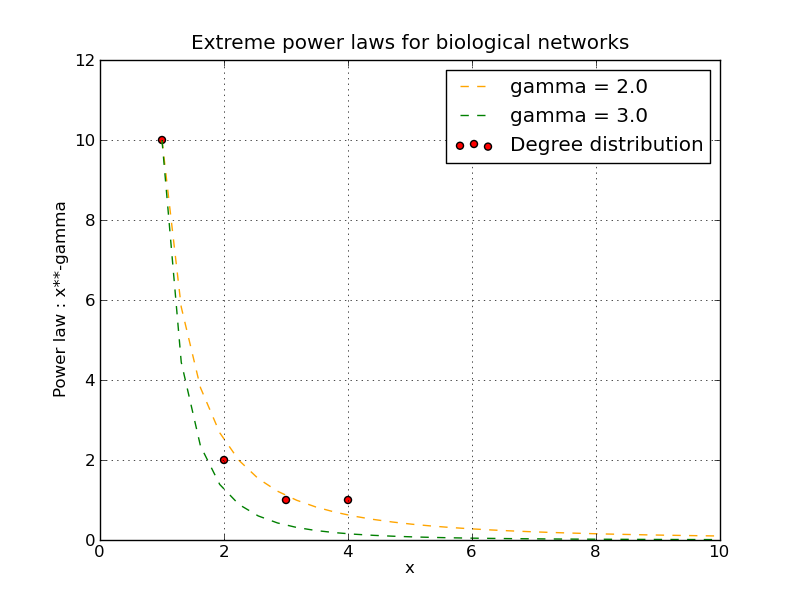
\includegraphics[width=0.50\textwidth]{Plot.png}
  \end{center}
  \caption{Distribution puissances limites}
  \label{scalefree}
\end{wrapfigure}
\paragraph*{Formation de cliques\\}

Un graphe compte un certain nombre de cliques de différentes tailles. Une clique est un ensemble de nœuds entièrement interconnectés. Le coefficient de clustering est un bon indicateur de la présence de cliques et se calcule pour chaque nœud de la manière suivante :
$$ C_i = \frac{2Ei}{k_i k_{i-1}} $$
avec
\begin{itemize}
 \item $E_i$ : nombre de liens entre voisins ;
 \item $k_i$ : nombre de voisins de $i$.
\end{itemize}
Nous allons utiliser le coefficient de clustering global, c'est-à-dire la moyenne des coefficients de chaque nœud. Ainsi, nous aurons une valeur comprise entre $0$ et $1$ que nous pourrons utiliser dans notre fonction de \textit{fitness}.



%%%%%%%%%%%%%%%%%%%%%%%%%%%%%%%%%
\section{Implémentation}
% Anthony

\subsection{Classes et objets}
% Anthony

\subsection{Codage d'un réseau}
% Anthony
\subsubsection{Matrice d'adjacence}
\subsubsection{Remplissage de la matrice}
\subsubsection{Fonctions}

\subsection{Algorithme génétique}
Nous utiliserons ici le module \texttt{AG.py} codée en scéances d'Optimisation. 

A chaque génération, on calcule la \textit{fitness} de chaque individu, qui est définie par une combinaison linéaire de coefficients témoignant de leur adéquation aux propriétés d'un réseau biologique (cf section \ref{fitness}).
Les individus sont classés en fonction de leur \textit{fitness}. On conserve les 10\% meilleurs individus pour la nouvelle génération. Ceux-ci subissent des mutations, des croisements, étapes fondamentales de l'évolution.

Une fois la génération finale obtenue, on teste la robustesse du meilleur réseau obtenu (conservation des propriétés malgré la suppression au hasard d'un nœud) ainsi que leur concordance avec la propriété de non-assortativité (les hubs ne sont pas reliés entre eux).

On lancera cette simulation plusieurs fois afin de mesurer le temps moyen de convergence.
Les paramètres finaux des réseaux type \og biologique \fg sont conservés afin de permettre un étude comparative. D'un simulation à une autre, nous feront varier la pondération des paramètres de la loi de \textit{fitness} et le degré de la loi de puissance, ce qui nous permettra d'étudier leur impact respectif.

\subsection{Fonction de \textit{fitness} }
\label{fitness}
La \textit{fitness} d'un individu est un nombre réel compris entre 0 et 1, 1 correspondant à une \textit{fitness} maximale.
Celle-ci est calculée comme une somme linéaire pondérée des résultats renvoyés par les fonctions \texttt{}, \texttt{}, et \texttt{}, testant l'adéquation du réseau aux paramètres principaux d'un réseau biologique : formation de cliques, distribution des degrés selon une loi de puissance et propriété de petit monde.

\medskip
Nous pondérons cette somme pour favoriser un critère par rapport aux autres. En effet, la coexistence de propriété de petit monde et de formation de clique est fondamentalement paradoxale. Sans ce favoritisme, l'émergence de réseaux biologique est fortement freinée, voir inhibée.

%Combinaison libéaire de fonction
%Pourquoi pondérer ?

%%%%%%%%%%%%%%%%%%%%%%%%%%%%%%%%%%%%%%%%%
\section{Planning}

\subsection{Répartition du travail}

\begin{center}
\begin{table}[!h]
\begin{tabular}{|c|c|c|}
\hline \textbf{Fonction} & \textbf{Attribué à} & \textbf{Date de rendu} \\
\hline
Adaptation de \verb?AlgoGen? & Marie & 03/04 \\
\hline
\verb?fit2distri()? & Balthazar & 31/03 \\
\hline
\verb?clustering()? & Marie & 01/04\\
\hline 
\verb?smallWorld()? & Marion & 01/04\\
\hline
\verb?fitness()? & Anthony & 03/04\\
\hline 
\verb?genome2adj()? & Balthazar & 31/03 \\
\hline 
\verb?graphPrint()? & Balthazar & 01/04 \\
\hline 
\verb?genoModif()? & Anthony & 03/04 \\
\hline 
\verb?robustness()? & Marion & 05/04 \\
\hline 
\verb?dissasortativity()? & Marion & 05/04\\
\hline 
\end{tabular}
\end{table}
\end{center}

Chacun est responsable de tester les fonctions qui lui sont attribuées avant la date de rendu. Ces tests se feront sur des graphes créés avec \verb?NetworX? (manuellement et de façon automatique : scale-free, aléatoire, etc. ) et des données biologiques.

\subsection{Exploitation}
Nous commençons par tester notre code sur une population de 50 individus, chacun composé de 15 nœuds. Ceci nous permet d'approximer le temps de convergence et ainsi de mieux ma\^itriser les délais d'exploitation.

Nous pouvons alors trouver un compromis entre taille de la population et nombre de nœuds dans un réseau. A priori, une population de 50 individus ayant chacun 100 nœuds nous semble un bon début. Ces paramètres seront à adapter en fonction du temps de calcul.

Après avoir lancé une simulation, Plusieurs simulations seront lancées en parallèle, chacune ayant des paramètres différents : taille de la population, taille d'un réseau, pondération de la fonction de \textit{fitness}, paramètre de la loi de puissance. Les résultats obtenus seront exploités en vue de déterminer leur influence respective sur la formation d'un réseau biologique.

\subsection{Risques}
Nous utilisons Python qui est un langage de haut niveau : le temps de calcul des fonctions proposées est a priori optimisé mais l'encapsulation ne permet pas sa maîtrise. De plus, nous utilisons pour la première fois le module \verb?NetworkX?. Bien que nous ne le ma\^itrisions pas parfaitement, une partie de notre code repose entièrement dessus. Nous ne connaissons donc pas les performances calcul de ce module.

Il est donc à craindre une mauvaise appréhension du temps de calcul liée à la taille de la population et des réseaux ainsi qu'à l'encapsulation de nombreuses fonction \verb?Python?.


\end{document}